% ---------------------------- %
% COM1005 Assignment Report
% 
% Rebanth Kanner, 2021
% --------------------------   %


\documentclass[11pt,oneside]{article}
\usepackage[utf8]{inputenc}
\usepackage{graphicx}
\usepackage{float}


\title{Experimental report for the 2021 COM1005 Assignment: The Rambler's Problem\footnote{https://github.com/RebanthK/COM1005_aca20rk.git}}
\author{Rebanth Kanner}
\date{\today}


\begin{document}

\maketitle

\section{Description of my branch-and-bound implementation}
For my Branch-and-Bound implementation, apart from the given classes (Search.java, SearchState.java, SearchNode.java, TerrainMap.java and Coords.java) I have written five more classes; CoordsLink, Carta, RamblersState (which extends the given abstract class SearchState), RamblersSearch(which extends the given abstract class Search) and RunRamblersBB which declares the start and end coordinates and runs the search.

\begin{itemize}
    \item CoordsLink.java is a class that takes in two coordinates(Coords objects) and their heights(integers) as parameters and calculates the cost(integer) when moving from the first coordinate to the second. It is used in Carta.java to construct the State Space where the search will take place.
    \item Carta.java is a class that constructs the State Space which is an ArrayList of CoordsLink objects. It does so by reading the TerrainMap object(the two dimensional array) returned by the TerrainMap.java class that has been given to us. It has methods that return the entire State Space, all the individual coordinates(Coords objects), as well as a method that return all the links of a specific inputted coordinate(Coords object), and a method to return the cost between two inputted coordinates(Coords objects).
    \item RamblersState.java is a class that extends SearchState.java and defines the constructor and accessor for a single state in the State space. It also implements the goalPredicate method (checking if the state of the current node is the goal state), the getSuccessors method (which calls the getlinks method in Carta.java to find the successor states to the current state), and the sameState method (which returns a boolean whether the two states are the same or not).
    \item The provided Search.java class consists of majority of the code that runs the search itself with the branch and bound method.
    \item RamblersSearch.java is a class that extends Search.java and constructs the Ramblers Search with the Carta Object(State Space) and the goal state as parameters.
    \item RunRamblersBB,java is the class that defines the list of start and end coordinates that we use to test the search algorithm and runs the search.
\end{itemize}

\section{Description of my A* implementation}
For the implementation of my A* Search I have made use of the same classes as that of Branch and Bound with slight or no modifications. 

\begin{itemize}
    \item CoordsLink.java, RamblersSearch.java, Search.java, SearchState.java,  SearchNode.java, TerrainMap.java and Coords.java remains the same as it was in the Branch-and-bound implementation.
    \item Carta.java also remains the same however with one extra method, estbetween. estbetween is used to calculate the estimated remaining cost between the current and goal nodes that is used in the A* search, based off different heuristics. For this study I have used five heuristics. They are:
        \begin{itemize}
            \item The Manhattan Distance
            \item The Euclidean Distance
            \item The Height Difference
            \item The Euclidean Distance + Height Difference
            \item The Manhattan Distance + Height Difference
        \end{itemize}
    
    \item RamblersState.java also remains the same for most part, however now instead of just storing the coordinates and the local cost from the previous state it also stores the estimated remaining cost.
    \item Search.java now uses the A* method when searching through the State Space
    \item RunRamblersAstart.java replaces RunRamblersBB.java to define the list of start and end coordinates that we use to test the search algorithm, and, run the search.
\end{itemize}
 
\section{Assessing efficiency}
To assess the efficiency of all the search algorithms a test was run with a set of 50 different coordinates through each algorithm and recording their efficiencies.

\subsection{Assessing the efficiency of my branch-and-bound search algorithm}
A sample of the data I have collected to assess the Branch-and-bound search is displayed below. The table consists of the Starting Coordinates(x,y), the goal coordinates(x,y), the cost of the path returned and the efficiency of that particular search. The average efficiency of all the tests conducted on the algorithm was 0.003494225.

\begin{table}[H]
    \centering
    \begin{tabular}{|c|c|c|c|}
        Start        & Goal       & Cost & Efficiency \\ \hline
        (125, 194)   & (100, 212) & 110 & 0.001267758 \\
        (178, 205)   & (100, 155) & 248 & 0.001267758 \\
        (200, 154)   & (193, 110) & 120 & 0.001267758 \\
        (210, 123)   & (145, 80)  & 193 & 0.001267758 \\
        (35, 216)    & (43, 200)  & 54 & 0.001267758 \\
        (93, 88)     & (73, 70)   & 45 & 0.001267758 \\
        (0, 0)       & (200, 200) & 568 & 0.001267758 \\
    \end{tabular}
    \caption{Sample Data Table for Branch and Bound Search Algorithm}
    \label{tab:my_label}
\end{table}

Figure~\ref{fig:BnBEvC} below displays a scatter-plot diagram plotting the efficiencies vs cost for the paths between the coordinates inputted into the branch-and-bound search algorithm. From the graph plotted and the line of best fit, we can identify that for paths with lower costs, below 50, the algorithm is considerably more efficient. This efficiency also falls off considerably for costs greater than 50.

\begin{figure}[H]
\centering
  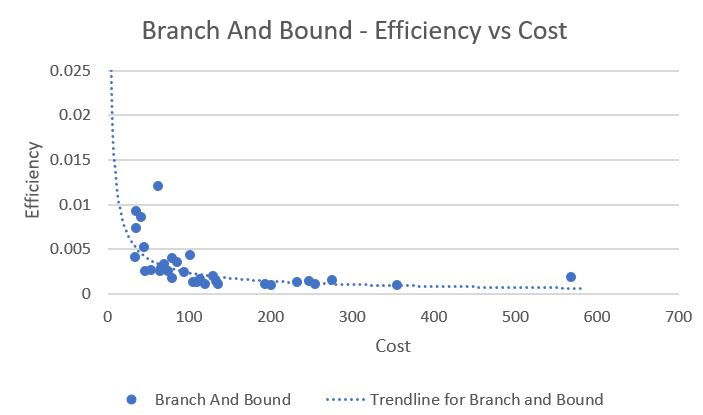
\includegraphics[scale=0.8]{BnB efficiency vs cost.JPG}
  \caption{The scatter-plot for branch and bound.}
  \label{fig:BnBEvC}
\end{figure} 

\subsection{Assessing the efficiency of my A* search algorithm}
For the A* algorithm I have investigated using 5 different heuristics, therefore creating 5 variations of the A* search algorithm

\subsubsection{The Manhattan Distance Heuristic}
    A sample of the data I have collected to assess the A* search algorithm using the Manhattan Distance Heuristic is displayed below. The table consists of the Starting Coordinates(x,y), the goal coordinates(x,y), the cost of the path returned and the efficiency of that particular search. The average efficiency of all the tests conducted on the algorithm was 0.040833194.
 
\begin{table}[H]
    \centering
    \begin{tabular}{|c|c|c|c|}
        Start        & Goal       & Cost & Efficiency \\ \hline
        (125, 194)   & (100, 212) & 110 & 0.004076339 \\
        (178, 205)   & (100, 155) & 248 & 0.002666226 \\
        (200, 154)   & (193, 110) & 120 & 0.004528828 \\
        (210, 123)   & (145, 80)  & 193 & 0.00458986 \\
        (35, 216)    & (43, 200)  & 54 & 0.015451174 \\
        (93, 88)     & (73, 70)   & 45 & 0.02895323 \\
        (0, 0)       & (200, 200) & 568 & 0.003088345 \\
    \end{tabular}
    \caption{Sample Data Table for the Manhattan distance heuristic of the A* Search Algorithm}
    \label{tab:my_label}
\end{table} 
    
    This heuristic performed much better than expected and even outperformed all but one of the other heuristics I have used in the A* search algorithm. It was almost 4 times as efficient as the Height Difference Heuristic, 2 times as efficient as the Euclidean Distance + Height difference heuristic, 9 times as efficient as the Euclidean Distance Heuristic but only 0.5 times as efficient as the Manhattan Distance + Height heuristic.
    
    Figure~\ref{fig:MDEvC} below displays a scatter-plot diagram plotting the efficiencies vs cost for the paths between the coordinates inputted into the A* search algorithm when using the Manhattan Difference Heuristic. It is worth noting that this graph has larger scale on the y-axis as compared to some of the other graphs. This is because it is considerably more efficient than the other algorithms, and while the efficiency falls off for costs greater than 100 it still has a higher efficiency than some of the other algorithms.

    \begin{figure}[H]
    \centering
      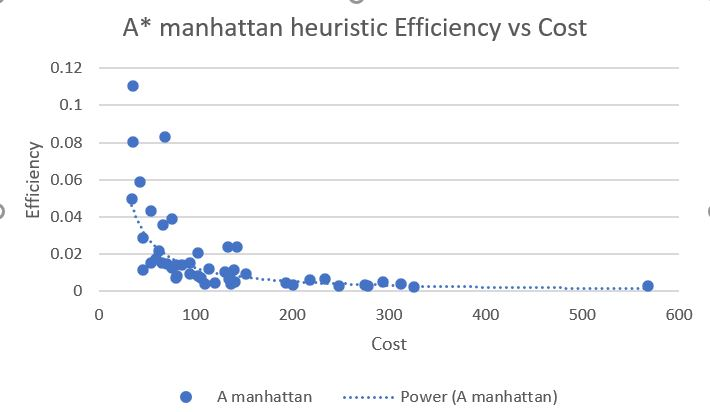
\includegraphics[scale=0.8]{MD efficiency vs cost.JPG}
      \caption{The scatter-plot for the Manhattan Distance Heuristic.}
      \label{fig:MDEvC}
    \end{figure} 

\subsubsection{The Euclidean Distance Heuristic}

A sample of the data I have collected to assess the A* search algorithm using the Euclidean Distance Heuristic is displayed below. The table consists of the Starting Coordinates(x,y), the goal coordinates(x,y), the cost of the path returned and the efficiency of that particular search. The average efficiency of all the tests conducted on the algorithm was 0.004385691. 

\begin{table}[H]
    \centering
    \begin{tabular}{|c|c|c|c|}
        Start        & Goal       & Cost & Efficiency \\ \hline
        (125, 194)   & (100, 212) & 110 & 0.004076339 \\
        (178, 205)   & (100, 155) & 248 & 0.002666226 \\
        (200, 154)   & (193, 110) & 120 & 0.004528828 \\
        (210, 123)   & (145, 80)  & 193 & 0.00458986 \\
        (35, 216)    & (43, 200)  & 54 & 0.015451174 \\
        (93, 88)     & (73, 70)   & 45 & 0.02895323 \\
        (0, 0)       & (200, 200) & 568 & 0.003088345 \\
    \end{tabular}
    \caption{Sample Data Table for the Euclidean distance heuristic of the A* Search Algorithm}
    \label{tab:my_label}
\end{table}

This Heuristic performed the worst amongst all the A* heuristics that I tested, being 0.25 times efficient as the Height difference + Euclidean Distance heuristic, 0.4 times efficient as the Height difference heuristic, 0.1  times efficient as the Manhattan Distance Heuristic and 0.05 times as efficient as the Manhattan distance + Height difference heuristic. 

Figure~\ref{fig:EDEvC} below displays a scatter-plot diagram plotting the efficiencies vs cost for the paths between the coordinates inputted into the A* search algorithm when using the Euclidean Difference Heuristic.

\begin{figure}[H]
    \centering
      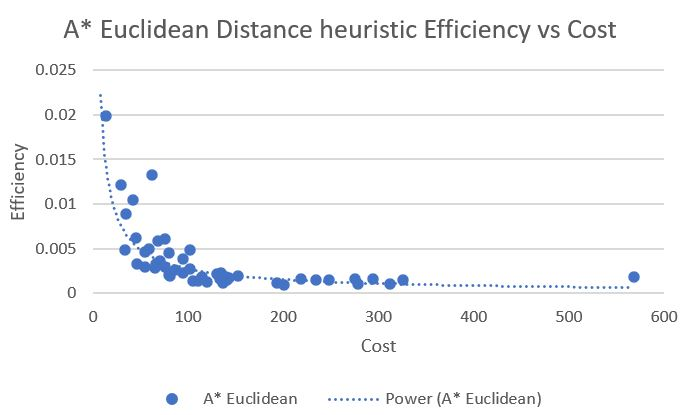
\includegraphics[scale=0.8]{ED efficiency vs cost.JPG}
      \caption{The scatter-plot for the Euclidean Distance Heuristic.}
      \label{fig:EDEvC}
    \end{figure} 

\subsubsection{The Height difference Heuristic}
A sample of the data I have collected to assess the A* search algorithm using the Height Difference Heuristic is displayed below in Table 3. The Height Difference heuristic simply returns the estimated remaining cost as the difference in height between the current and goal coordinates. The table consists of the Starting Coordinates(x,y), the goal coordinates(x,y), the cost of the path returned and the efficiency of that particular search. The average efficiency of all the tests conducted on the algorithm was 0.010362525. 

\begin{table}[H]
    \centering
    \begin{tabular}{|c|c|c|c|}
        Start        & Goal       & Cost & Efficiency \\ \hline
        (125, 194)   & (100, 212) & 110 & 0.006869633 \\
        (178, 205)   & (100, 155) & 253 & 0.001817174 \\
        (200, 154)   & (193, 110) & 120 & 0.002199755 \\
        (210, 123)   & (145, 80)  & 198 & 0.001167749 \\
        (35, 216)    & (43, 200)  & 54 & 0.004841209 \\
        (93, 88)     & (73, 70)   & 45 & 0.012678804 \\
        (0, 0)       & (200, 200) & 569 & 0.001953857 \\
    \end{tabular}
    \caption{Sample Data Table for the Height Difference heuristic of the A* Search Algorithm}
    \label{tab:my_label}
\end{table}

It should be noted that on observing the data collected on a few instances this heuristic in some instances returned paths that were more costly by 1-5 units and in others returned efficiencies that were higher than the Manhattan Distance heuristic. However, on average this heuristic was 0.25 times as efficient as the Manhattan Distance Heuristic, 0.5 times as efficient as the Height+Euclidean Distance heuristic, 2.3 times as efficient as the Euclidean Distance Heuristic and 0.125 times efficient as the Manhattan Distance + Height Difference Heuristic.

Figure~\ref{fig:HDEvC} below displays a scatter-plot diagram plotting the efficiencies vs cost for the paths between the coordinates inputted into the A* search algorithm when using the Height Difference Heuristic. As seen in the scatter-plot, similar to all the other A* algorithms the efficiency greatly falls off when the cost increases above 100 units.

\begin{figure}[H]
    \centering
      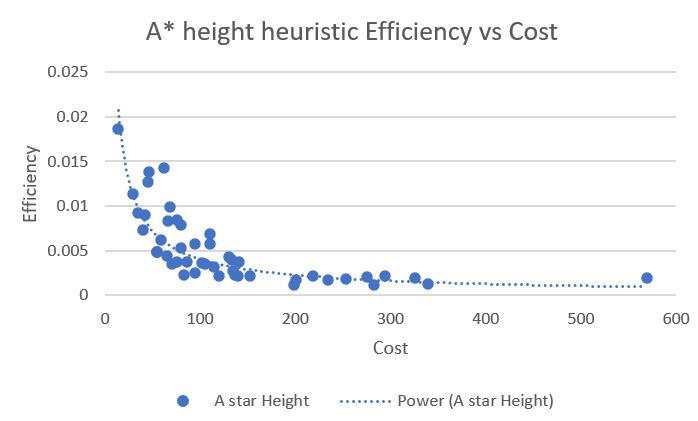
\includegraphics[scale=0.8]{HD efficiency vs cost.JPG}
      \caption{The scatter-plot for the Height Difference Heuristic.}
      \label{fig:HDEvC}
    \end{figure} 

\subsubsection{Mixed Heuristic, Height+Euclidean Distance}
A sample of the data I have collected to assess the A* search algorithm using the Euclidean Distance + Height Difference Heuristic is displayed below. The table consists of the Starting Coordinates(x,y), the goal coordinates(x,y), the cost of the path returned and the efficiency of that particular search. The average efficiency of all the tests conducted on the algorithm was 0.018385558. It is also worth noting that in some instances the algorithm using this heuristic returned paths that were more costly by 1 - 7 units.

\begin{table}[H]
    \centering
    \begin{tabular}{|c|c|c|c|}
        Start        & Goal       & Cost & Efficiency \\ \hline
        (125, 194)   & (100, 212) & 110 & 0.008512285 \\
        (178, 205)   & (100, 155) & 253 & 0.001887045 \\
        (200, 154)   & (193, 110) & 120 & 0.002634403 \\
        (210, 123)   & (145, 80)  & 193 & 0.001209874 \\
        (35, 216)    & (43, 200)  & 54 & 0.005523641 \\
        (93, 88)     & (73, 70)   & 45 & 0.015931373 \\
        (0, 0)       & (200, 200) & 569 & 0.002011608 \\
    \end{tabular}
    \caption{Sample Data Table for the Euclidean distance + Height Difference heuristic of the A* Search Algorithm}
    \label{tab:my_label}
\end{table}

This heuristic was 4 times as efficient as the Euclidean Distance and 1.7 times as efficient as the height difference heuristic, 0.22 times efficient as the Manhattan Distance + Height heuristic, and was surprisingly only 0.5 times efficient as the Manhattan Distance heuristic.

Figure~\ref{fig:EDHDEvC} below displays a scatter-plot diagram plotting the efficiencies vs cost for the paths between the coordinates inputted into the A* search algorithm when using the Euclidean Distance + Height Difference Heuristic. The efficiency of the search algorithm using this heuristic also falls off 
\begin{figure}[H]
    \centering
      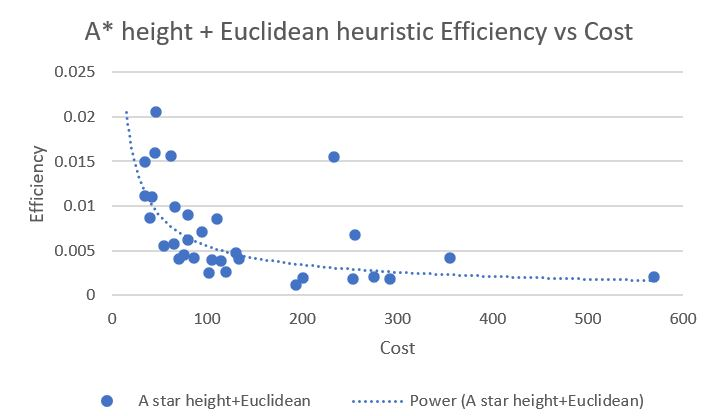
\includegraphics[scale=0.8]{ED+HD efficiency vs cost.JPG}
      \caption{The scatter-plot for the Euclidean Distance + height difference Heuristic.}
      \label{fig:EDHDEvC}
    \end{figure} 
    
\subsubsection{Mixed Heuristic, Height+Manhattan Distance}
A sample of the data I have collected to assess the A* search algorithm using the Manhattan Distance + Height Difference Heuristic is displayed below. The table consists of the Starting Coordinates(x,y), the goal coordinates(x,y), the cost of the path returned and the efficiency of that particular search. The average efficiency of all the tests conducted on the algorithm was 0.082665588.

\begin{table}[H]
    \centering
    \begin{tabular}{|c|c|c|c|}
        Start        & Goal       & Cost & Efficiency \\ \hline
        (125, 194)   & (100, 212) & 113 & 0.07470289 \\
        (178, 205)   & (100, 155) & 256 & 0.00336885 \\
        (200, 154)   & (193, 110) & 121 & 0.011223829 \\
        (210, 123)   & (145, 80)  & 198 & 0.004245044 \\
        (35, 216)    & (43, 200)  & 54 & 0.020424837 \\
        (93, 88)     & (73, 70)   & 48 & 0.10512129 \\
        (0, 0)       & (200, 200) & 599 & 0.002885598 \\
    \end{tabular}
    \caption{Sample Data Table for the Manhattan distance + Height Difference heuristic of the A* Search Algorithm}
    \label{tab:my_label}
\end{table}

On average this heuristic was 2 times as efficient as the Manhattan Distance Heuristic, 4.5 times as efficient as the Height+Euclidean Distance heuristic, 18.8 times as efficient as the Euclidean Distance Heuristic and 8 times efficient as the Height Difference Heuristic. However, while this algorithm on average was most efficient, there were instances where it returned costs of routes that were much higher than other heuristics.

Figure~\ref{fig:MDHDEvC} below displays a scatter-plot diagram plotting the efficiencies vs cost for the paths between the coordinates inputted into the A* search algorithm when using the Manhattan Distance + Height Difference Heuristic. It should be noted that this graph has a y-axis scale that is much larger than the others, since it is significantly more efficient. The efficiency of the search algorithm using this heuristic also falls off when the cost increases above 100 units.

\begin{figure}[H]
    \centering
      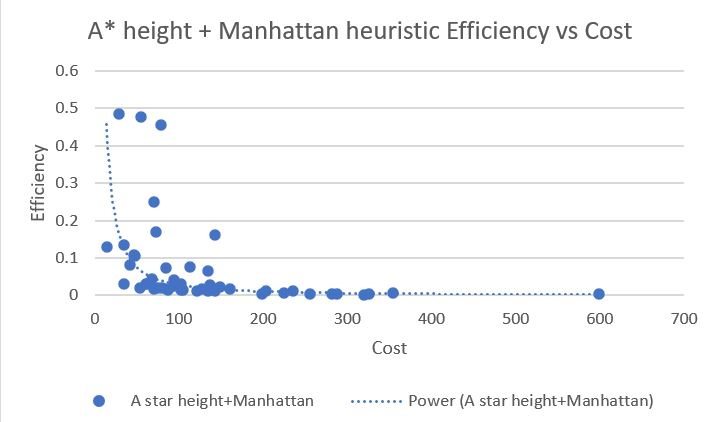
\includegraphics[scale=0.8]{MD+HD efficiency vs cost.JPG}
      \caption{The scatter-plot for the Manhattan Distance + height difference Heuristic.}
      \label{fig:MDHDEvC}
    \end{figure} 
    
\subsubsection{Comparing the A* heuristics}
On observation the efficiencies of the A* algorithm using each heuristic is ranked as following from highest to lowest efficiencies.

\begin{itemize}
    \item Manhattan Distance + Height Difference heuristic
    \item Manhattan Distance heuristic
    \item Euclidean Distance + Height Difference heuristic
    \item Height Difference heuristic
    \item Euclidean heuristic
\end{itemize}

An A* search becomes admissible only if the estimated remaining costs are all accurate or all underestimates, which is true in the case of all the heuristics. However the higher the underestimate (the closer the estimate is to the actual remaining cost), the more efficient the search algorithm is.

Height difference and Euclidean distance individually both had the lowest efficiencies. This could be because these heuristics returned underestimates that were too low to be entirely viable. In fact they were so low that even a combination of the two was more inefficient than the Manhattan distance individually.

The reason the Manhattan Distance + Height heuristic works best can be traced to the path the RamblersSearch takes. The Manhattan distance is essentially the shortest number of nodes to the goal state without considering the height. The Manhattan distance provides a better estimate than the Euclidean distance as the Ramblers Search algorithm cannot move in the direction of the Euclidean Distance, and can only move up, down, left or right towards other nodes. Since Height is also a part of the cost in the main algorithm, this heuristic was added to the Manhattan Distance, to produce the Mixed heuristic of Manhattan Distance + Height. However there are certain drawbacks in this heuristic. As stated before there were instances where the cost of the route was higher than costs returned by other heuristics. This is probably because the height heuristic might be misled by local maxima and minima, and therefore may end up taking a longer route.

\subsection{Comparing the two search strategies}
According to the observations made by running the test pairs of start and end coordinates it is clear that all A* strategies(all heuristics) outperformed the branch-and-bound strategy. This however was expected as the branch-and-bound strategy is a form of uninformed search, and is essentially searching blindly in all directions, while the informed A* search strategy has a sense of "direction", towards which it searches. However, efficiency aside both searches are certainly admissible and will find the goal coordinates.

For the comparison of values I will be using the best heuristic from those that have been investigated, that is the Manhattan Distance + height heuristic. As stated before, the A* search strategy had an efficiency of 0.082665588 while the branch and bound search had an efficiency of 0.003494225. This means on average the A* search was 23.6 times more efficient that the branch-and-bound search algorithm. However it should be noted that in some cases, the A* search did return costs that were slightly higher than the branch-and-bound, but there were also cases where the costs returned by the branch-and-bound algorithm were much higher than the A* algorithm. One aspect that remained common for both algorithms(regardless of heuristic in the case of A*) was that their efficiencies began to fall off when the cost was above 100.

\section{Conclusions}
All the data collected and observations made, were within my expectations, supporting the fact that informed A* searches are several times more efficient than uninformed branch-and-bound searches. The results also prove that both searches are admissible even with varying efficiencies. With regard to the efficiencies of the heuristics of the A* search, it was slightly unexpected that the Mixed Heuristic of Euclidean Distance + Height difference was less efficient than the Manhattan Distance heuristic, however upon a closer inspection, it too was justifiable.

\end{document}
